\chapter{Conclusion}
\label{ch:conclusion}
This chapter discuss the query expansion implementation and compares it to Rudihagen's implementation.
Lastly, the writer suggest possible improvements to futher increase performance.

\section{Discussion}
[Elasticsearch will return the photos which have most hits on the terms search for]

Figure \ref{fig:sequence-diagram-search-master} shows the sequence diagram for Rudihagen's query expansion solution using KL.
On the figure 4 round trips are required from the webserver to the database and the search engine.
The implementation discussed in Chapter \ref{ch:approach} describes a solution to decrease the number of round trips from 4 to 2.
In Chapter \ref{ch:evaluation} the performance is greatly increased.

\begin{figure}[h!]
\centering 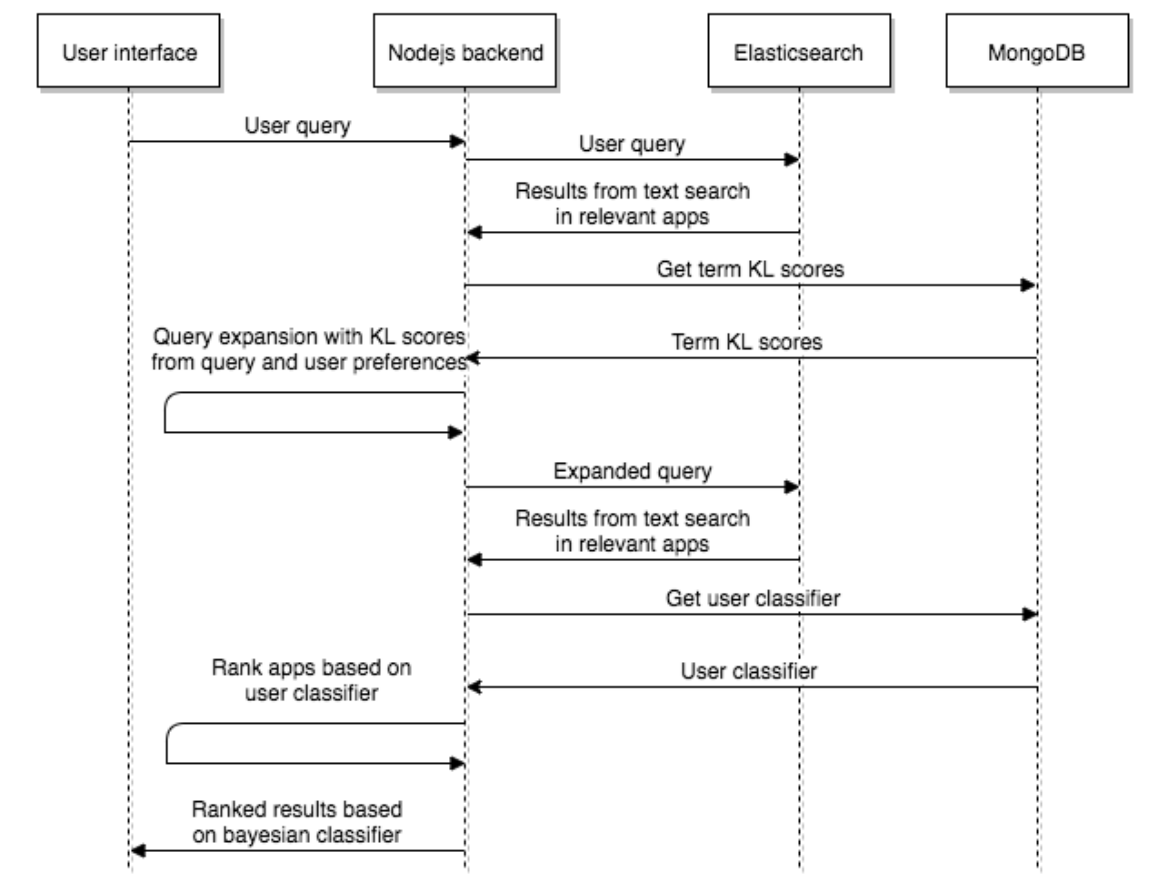
\includegraphics[width=0.9\linewidth]{img/sequence-diagram-search-master-thesis.png}
\caption{Sequence diagram from Rudihagen's master thesis implementation of query expansion using KL \cite[p. 37]{master-thesis}.}
\label{fig:sequence-diagram-search-master}
\end{figure}

Even though the latency was greatly reduced there are a few disclamers.
Firstly both the webserver and the search engine ran on the same computer.
As a result the round trip time was almost negligible, which is often not the case in a real world environment.
To give more realistic measurements, the solution should be tested on a cloud solution where the webserver and the search engine doesn't run on the same physical server.

\section{Futher Work}
After implementing a query expansion which requires two round trips there is still room for improvement.
The writer suggested to explore the two following solutions to avoid the extra round trip:

\begin{itemize}
    \item Use Elasticsearch's scripting functionality to evaluate custom expressions \footnote{\url{https://www.elastic.co/guide/en/elasticsearch/reference/current/modules-scripting.html}}.
    \item Implement query expansion in Lucene.
\end{itemize}
